\documentclass[tikz,border=10pt]{standalone}
% Shared look for every TikZ diagram. Load with \input{../../tools/tikz-style.tex}
\usepackage[T1]{fontenc}
\usepackage{lmodern}
\renewcommand{\sfdefault}{lmr}  % diagrams use the same serif as the text
\usetikzlibrary{arrows.meta, positioning, shapes.geometric, calc, fit, backgrounds}
\definecolor{cblue}{HTML}{4C78A8}
\definecolor{corange}{HTML}{F58518}
\definecolor{cgreen}{HTML}{54A24B}
\definecolor{cred}{HTML}{E45756}
\definecolor{cpurple}{HTML}{B279A2}
\definecolor{cgrey}{HTML}{6B6B6B}
\tikzset{
  every picture/.style={font=\sffamily, line width=1.2pt},
  box/.style={draw=#1, fill=#1!12, rounded corners=4pt, align=center, inner sep=7pt, minimum height=1.1cm},
  box/.default=cgrey,
  arrow/.style={-{Stealth[length=3mm]}, draw=cgrey, line width=1.4pt},
  title/.style={font=\sffamily\bfseries\Large},
  note/.style={font=\sffamily\small, text=cgrey, align=center},
}
\AtBeginDocument{\hyphenpenalty=10000 \exhyphenpenalty=10000}

\begin{document}
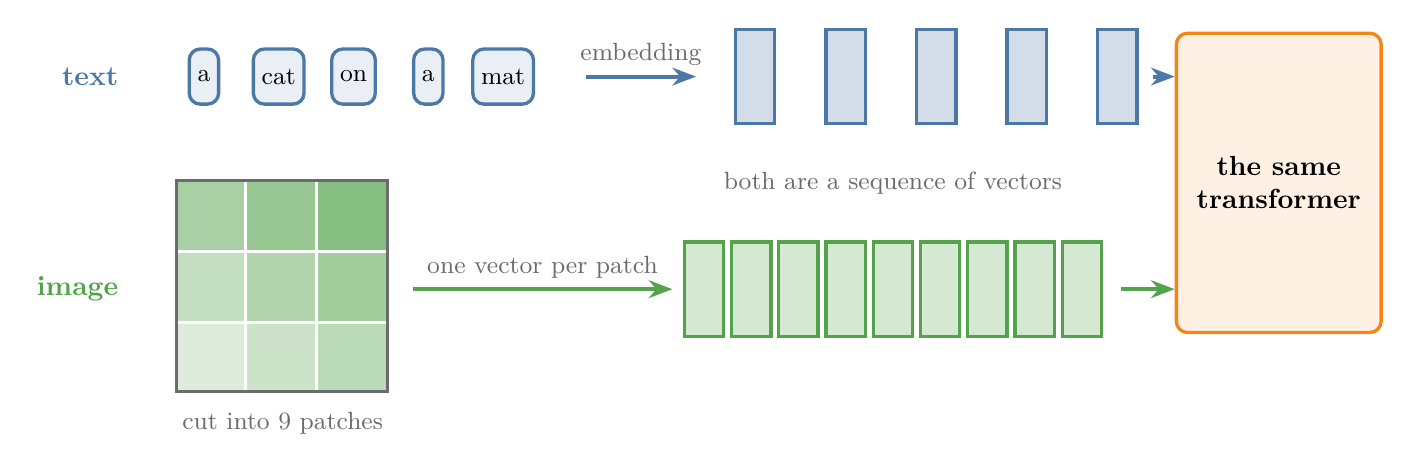
\begin{tikzpicture}[v/.style={draw=#1, fill=#1!25, minimum width=0.5cm, minimum height=1.2cm, inner sep=0pt}]
  % text row
  \node[anchor=east, font=\sffamily\bfseries, text=cblue] at (-0.4,2.4) {text};
  \foreach \w [count=\k] in {a, cat, on, a, mat} {
    \node[box=cblue, inner sep=3pt, minimum height=0.7cm, font=\sffamily\small] (w\k) at (0.95*\k-0.4,2.4) {\w};
    \node[v=cblue] (tv\k) at (1.15*\k+6.4,2.4) {};
  }
  \draw[arrow, draw=cblue] (5.4,2.4) -- node[above, note] {embedding} (6.8,2.4);
  % image row
  \node[anchor=east, font=\sffamily\bfseries, text=cgreen] at (-0.4,-0.3) {image};
  \foreach \i in {0,1,2} \foreach \j in {0,1,2} {
    \pgfmathsetmacro\shade{20+10*\i+15*\j}
    \fill[cgreen!\shade] (0.2+0.9*\i,-1.6+0.9*\j) rectangle ++(0.86,0.86);
  }
  \draw[cgrey] (0.2,-1.6) rectangle (2.88,1.08);
  \node[note] at (1.55,-2.0) {cut into 9 patches};
  \foreach \k in {1,...,9} \node[v=cgreen] (iv\k) at (0.6*\k+6.3,-0.3) {};
  \draw[arrow, draw=cgreen] (3.2,-0.3) -- node[above, note] {one vector per patch} (6.5,-0.3);
  % transformer
  \node[box=corange, minimum width=2.6cm, minimum height=3.8cm, font=\sffamily\bfseries] (tr) at (14.2,1.05) {the same\\transformer};
  \draw[arrow, draw=cblue] (12.6,2.4) -- (tr.west |- 0,2.4);
  \draw[arrow, draw=cgreen] (12.2,-0.3) -- (tr.west |- 0,-0.3);
  \node[note] at (9.3,1.05) {both are a sequence of vectors};
\end{tikzpicture}
\end{document}
